% !TEX root = ../main.tex
\section{Threat Model}


\begin{figure*}[pt]
	\centerline{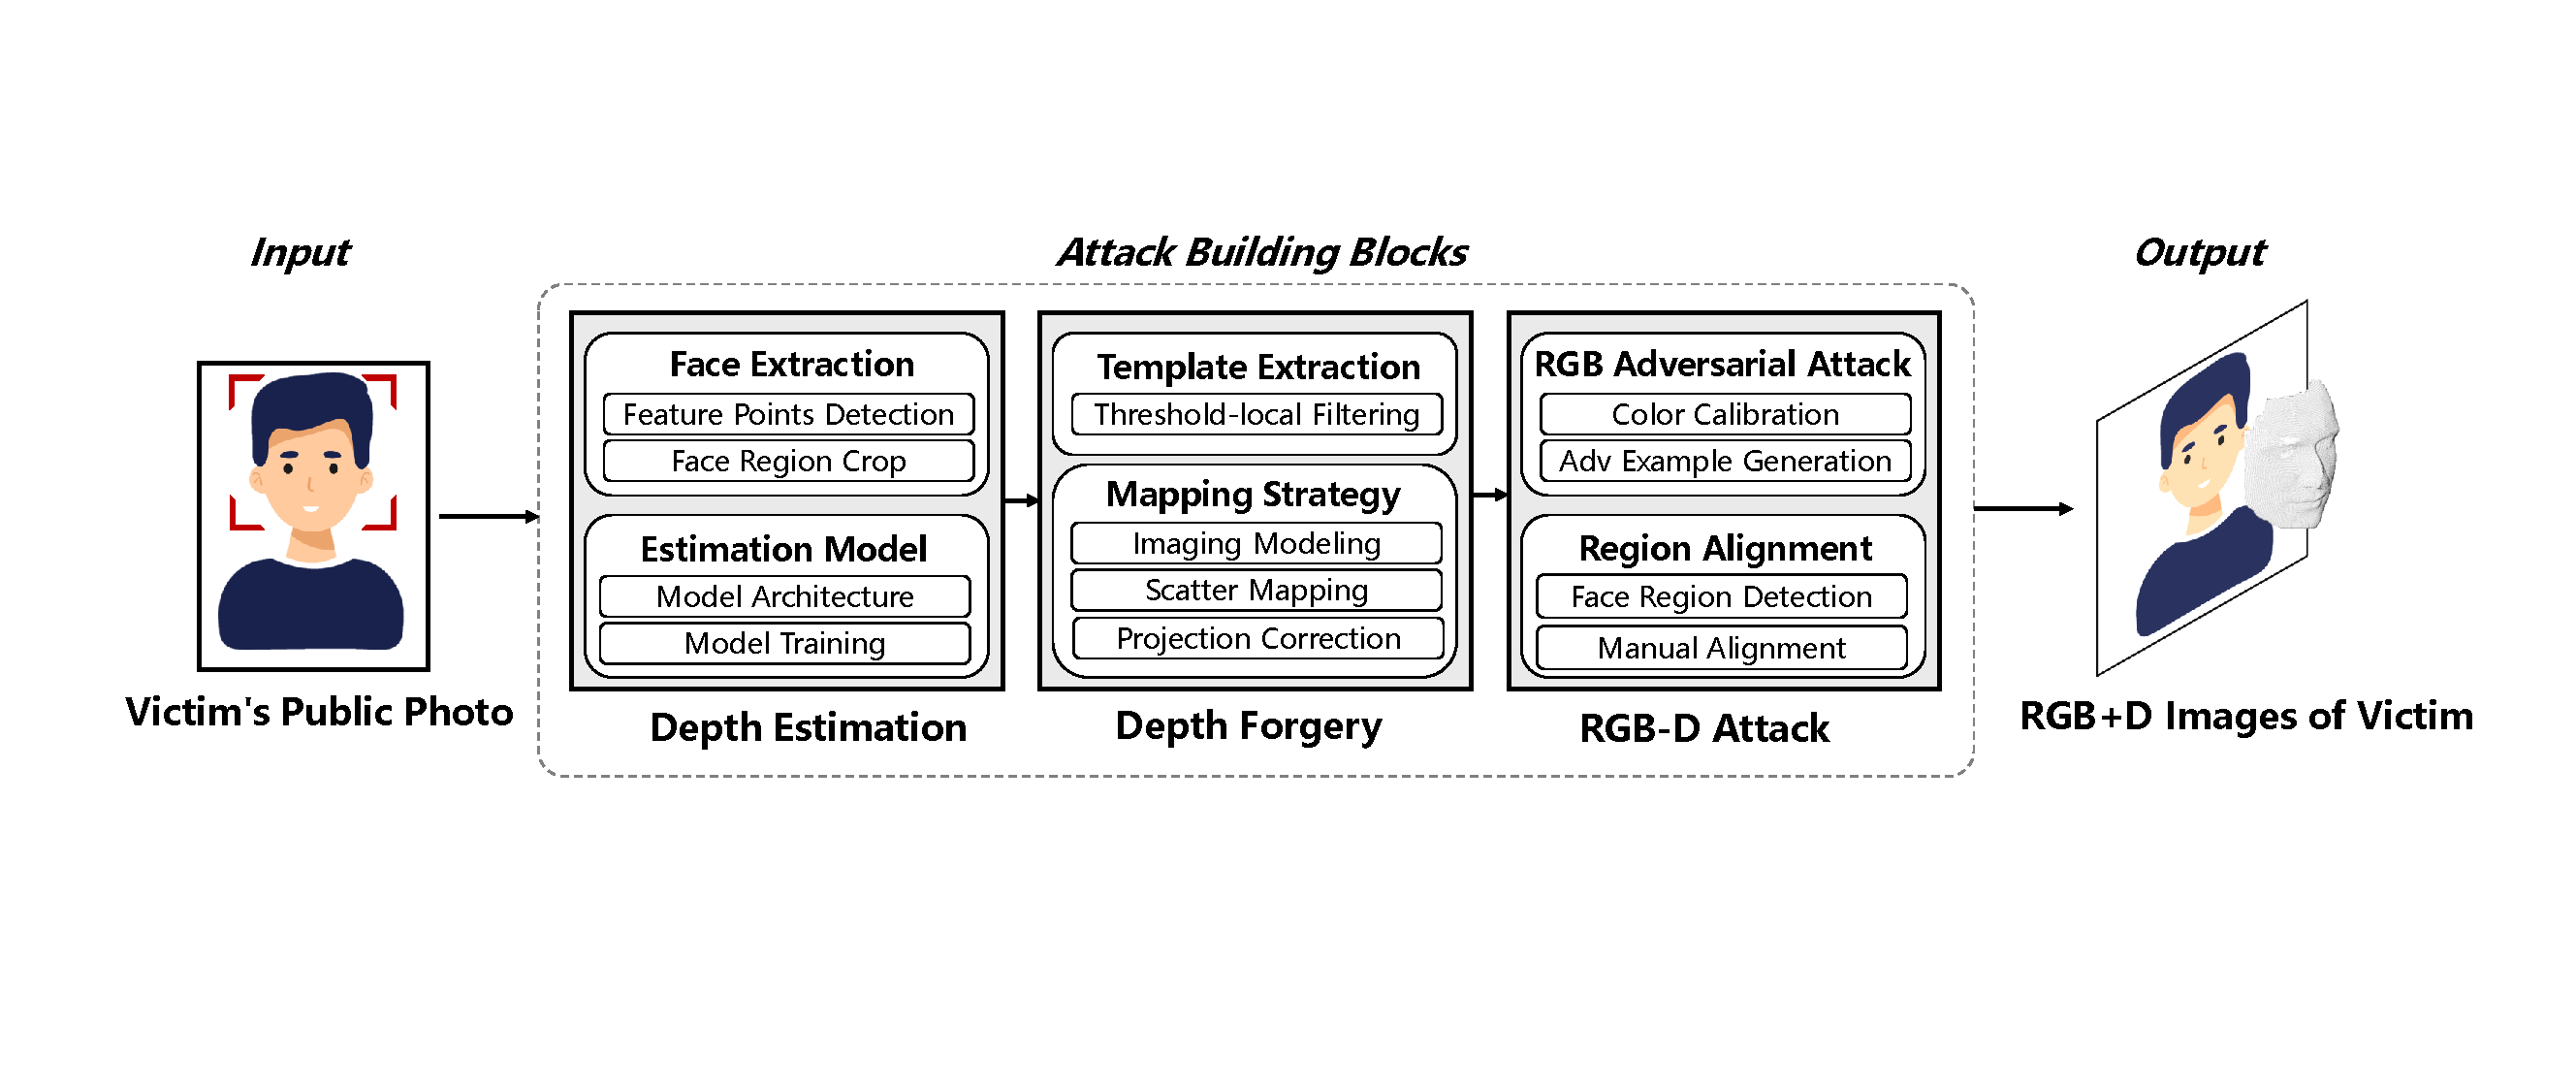
\includegraphics[width = \textwidth]{figures/overview.pdf}}
	\vspace{-0.1in}
	\caption{Overview of \texttt{DepthFake} attack: The adversary first estimates the depth image from the victim's 2D photo. Then, she extracts the template scatter pattern and modulates the depth information to the desired scatter pattern. When the RGB-D liveness detection is deployed, she uses the RGB adversarial attack and aligns it with the forgery depth image to launch a uniformed RGB-D attack.}
	\label{overview}
	\vspace{-0.15in}
\end{figure*}

The goal of the \texttt{DepthFake} attack is to spoof a 3D face authentication system using a 2D photo by bypassing its 3D liveness detection module. We consider the following attack scenario: An adversary wants to get inside a confidential place where the access control device is equipped with  a 3D face authentication system. To achieve it, she launches the \texttt{DepthFake} attack by placing the target victim's printed photo in front of the camera of the authentication system, as shown in Fig.~\ref{intro} and projecting the crafted-design scatter pattern onto the printed photo to spoof the 3D face authentication system to get access to the place.
%In this paper, we conduct two type of attacks as following: 
%
%\textbf{Depth Attack.} 
%
%\textbf{RGB-D Attack.} 

% The goal of \texttt{DepthFake} attack is to spoof the 3D face authentication system using a printed  photo by bypassing its 3D liveness detection module. Imaging a scenario where an adversary wants to get inside a confidential location where the 3D face authentication is deployed, or a scenario where the adversary wants to unlock a victim's smartphone which uses 3D face authentication. In either scenario, the adversary launches the \texttt{DepthFake} attack by projecting the deliberately crafted structured-light scatter pattern on an the photo of the victim user.

To achieve the aforementioned attack, we assume the adversary has the following capabilities:

\textbf{Depth Camera Awareness.}
The adversary can acquire a depth camera of the same model as the one used in the victim system. The attackers can obtain the template scatter pattern of the victim system by measuring that of the substitute camera.


\textbf{Public Photo Access.}
The adversary can obtain a  2D photo of the victim from  public platforms such as his social medias like Facebook, Twitter, WeChat, etc.
%\textbf{Camera and User Information Awareness.} 
%The adversary can acquire a depth camera of the same model as the one used in the victim system. Then, the adversary can utilize the camera to capture the template scatter pattern. Besides, the adversary can obtain the victim's 2D photo from the public platforms such as his social media or public databases.
%The adversary can acquire a camera of the same model as the one used in the victim system. Then, the adversary can utilize the camera to capture an RGB image and a depth image of the legitimate user.

\textbf{Physical Access to the Victim Device.} The adversary can physically get close to the victim system and set up the attack device, i.e., the printed photo displayed on a board and the infrared projector.


\textbf{Black-box Attack Setting.} 
We assume a black-box attack setting. For the depth forgery attack, the adversary does not require any output feedback from the victim system. While for the attack against the RGB image comparison, we assume she can obtain the  confidence score from the victim system as much prior work did~\cite{guo2019simple}.

% When deploying \texttt{DepthFake}, we only need to obtain the authentication results from the authentication system during the estimation and projection of the depth image. However, when the authentication system is extended to RGB-D mode, the adversary should also obtain the corresponding confidence scores of liveness detection. And there is no need to acquire prior knowledge of the authentication system, i.e., network architecture, parameters, etc. This is reasonable, as various commercial face authentication SDKs or APIs such as Tencent Cloud and Baidu Cloud only provide detection results or confidence scores, without exposing the model.


